% ============================================================================
% AI / Machine Learning contribution -- Paper 2: regional application and
% comparison. Companion to geosite_ai_section_2026.tex (Paper 1, national
% scale). Written 2026-08-23, restructured 2026-08-23 per full approved
% design plan (reference map, methodology tables, modified Table 1, gap
% charts, per-region + merged-group maps, national mosaic map).
%
% Content split per the supervisor-approved article plan (2026-08-21 PV):
% 20% literature review (brief context, this document's Section 2), 80% AI
% application per region with comparative performance/robustness/limitations
% analysis (Sections 3-6), core of the article, target ~15 pages.
%
% Every number in this section is drawn from a specific, verified source file
% in results/ (see inline "Source:" notes). Per user's explicit 2026-08-23
% instruction, results here are NOT gated behind McNemar significance testing
% the way Paper 1's national numbers are -- raw comparative numbers are
% reported directly.
% ============================================================================
\documentclass[11pt,a4paper]{article}
\usepackage[utf8]{inputenc}
\usepackage[T1]{fontenc}
\usepackage{amsmath}
\usepackage{amssymb}
\usepackage{graphicx}
\usepackage{booktabs}
\usepackage{array}
\usepackage{multirow}
\usepackage{colortbl}
\usepackage{hyperref}
\usepackage{float}
\usepackage{geometry}
\usepackage{xcolor}
\usepackage{microtype}
\usepackage{titlesec}
\usepackage{caption}
\usepackage[numbers]{natbib}
\usepackage{newpxtext}
\usepackage{newpxmath}
\usepackage[scaled=0.90]{helvet}
\usepackage{enumitem}

\geometry{a4paper, left=25mm, right=25mm, top=25mm, bottom=28mm, footskip=12mm}
\definecolor{accent}{HTML}{2B5F72}
\definecolor{groupbg}{HTML}{EDF2F3}
\hypersetup{colorlinks=true, linkcolor=accent, citecolor=accent, urlcolor=accent}
\raggedbottom
\setlength{\parindent}{0pt}
\setlength{\parskip}{6pt}

\titleformat{\section}{\normalsize\bfseries\sffamily\color{accent}}{\thesection}{0.8em}{}
\titleformat{\subsection}{\small\bfseries\sffamily}{\thesubsection}{0.8em}{}
\titlespacing*{\section}{0pt}{14pt}{6pt}
\titlespacing*{\subsection}{0pt}{10pt}{4pt}

\captionsetup{font=small, labelfont={bf,sf}, labelsep=period}
\renewcommand{\arraystretch}{1.15}

\newcommand{\headrule}{\vspace{-2pt}{\color{accent}\rule{\linewidth}{1pt}}\vspace{4pt}}

\begin{document}

% ---------------------------------------------------------------- Title ----
\begin{center}

\includegraphics[width=0.44\linewidth]{um6p_figures/um6p_gsmi_logo.png}\\[12pt]
{\color{accent!35}\rule{0.32\linewidth}{0.5pt}}\\[13pt]
{\LARGE\bfseries\sffamily Machine Learning Assessment of Geosite Accessibility in Morocco: Regional Application and Comparison}\\[6pt]
{\normalsize EL GORRIM Mohamed$^{1}$}\\[2pt]
{\small\itshape $^{1}$Geology and Sustainable Mining Institute (GSMI), Mohammed VI Polytechnic University (UM6P)}\\[2pt]
{\small Supervised by Dr.\ Ismail BEN AMAR, Sanae EL HARCHE, Mohamed EL OUALI}
\end{center}
\headrule

\begin{abstract}
\noindent\small
Companion to a national-scale assessment of geosite accessibility in Morocco, this paper applies the same terrain/infrastructure feature stack and validation protocol at regional scale, across ten region groupings covering 939 labeled geosites, with an explicit comparative focus on performance, robustness, and limitations that a single pooled national model cannot show. Unlike the national model, which uses one fixed six-feature set everywhere, each region here is allowed its own best-performing feature set among three candidates (a six-feature terrain/road baseline, the baseline plus geological domain, and the baseline plus tourism-infrastructure indicators) -- a region-specific methodology motivated by a direct empirical finding: no single feature set is best everywhere, and forcing one degrades some regions to improve others. Results range from strong, clearly above-baseline regional models (Marrakech-Safi Easy, +19.0 percentage points; the merged Guelmim-Oued Noun/Laâyoune-Sakia El Hamra group, +31.8 points) to regions where even the best available feature set cannot clear the local majority-class baseline (Marrakech-Safi Difficult, Béni Mellal-Khénifra Difficult). Three small regions, individually too thin to model, are shown to become usable once merged with a geographic neighbor. Every region's and merged group's best-model result is projected onto its own geographic grid and shown as a map, and these are combined into a single national mosaic covering eleven of Morocco's twelve regions (Oriental excluded for having zero labeled sites in the underlying catalog). A dedicated robustness analysis traces the recurring difficulty in the Difficult class to a specific, evidenced mechanism -- one region's terrain signature dominating the labeled training data -- rather than leaving it as an unexplained weakness, and situates today's per-region feature-selection result against a full day of ruled-out and partially-confirmed alternatives.
\end{abstract}

\section{Introduction}
The national-scale companion paper to this one asks whether accessibility is predictable from terrain and infrastructure data pooled across all of Morocco at once. Pooling eleven administratively and geologically distinct regions into a single feature space is, by construction, a compromise: it keeps the model spatially transferable, but it cannot show where the underlying approach works well, where it does not, and why. This paper is the detailed answer to that second question -- a systematic, region-by-region application and comparison, treating each region as its own modeling problem rather than a slice of a national average, and culminating in a single national map (Section~\ref{sec:mosaic}) assembled entirely from these region-specific results rather than from one pooled model.

\section{Regional Context}
\label{sec:regional-context}
Morocco is divided into twelve administrative regions (Figure~\ref{fig:regions-reference}), which form the organizing unit for every result in this paper. Morocco's geoheritage inventory spans terrain as varied as the flat, arid Saharan coastal plains of the south and the High and Middle Atlas mountain fronts in the center-north, with documentation density itself highly uneven -- geoheritage assessment has historically concentrated around the Fés-Meknés and Middle Atlas corridor, leaving southern and eastern regions comparatively under-surveyed. This regional imbalance in the underlying literature is itself a finding relevant to interpreting the results below (Section~\ref{sec:robustness}), not merely a data-collection footnote: several of the weakest regional results in this paper trace directly to how little of the existing published record covers that region, rather than to any property of the terrain itself.

\begin{figure}[H]
\centering
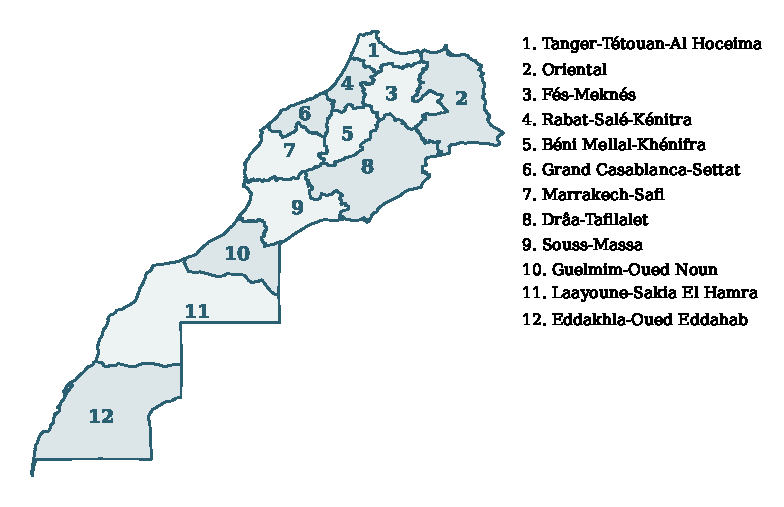
\includegraphics[width=0.62\linewidth]{figures/map_regions_reference.pdf}
\caption{Morocco's twelve official administrative regions, numbered for reference throughout this paper. Region 2 (Oriental) carries zero labeled geosites in the underlying catalog and is not modeled (Section~\ref{sec:mosaic}).}
\label{fig:regions-reference}
\end{figure}

\section{Methodology}
\label{sec:methodology}
The predictor variables, labeling protocol, and modeling algorithms are identical to the national companion paper; this section repeats only what is specific to the regional application -- the per-region feature-set choice and the region-merging rule -- and states the algorithms and validation protocol explicitly for a self-contained methodology section.

\subsection{Algorithms and Validation}
The deployed model, at every region and for every result reported below, is the same four-member soft-voted tree ensemble used nationally: Random Forest, XGBoost, Gradient Boosting, and LightGBM, trained with class-balance-weighted samples, with the best hyperparameter configuration for each of the four chosen once by grid search on the region's full labeled data. Section~\ref{sec:per-algorithm} additionally reports each of the four algorithms individually, rather than only the ensemble vote, as an explicit comparative view. Validation throughout is 500\,m haversine-clustered leave-one-group-out (LOGO) cross-validation: every labeled site within 500\,m of another is grouped into a single cluster, and an entire cluster is always held out together during testing, so that no model can score well merely by copying the label of a near-duplicate site it has effectively already seen. This is the same protocol used in the national companion paper, applied here separately within each region or merged group rather than once across the pooled national sample.

\subsection{Predictor Variables and Feature-Set Variants}
\label{sec:feature-variants}
Rather than applying one fixed feature set to every region, three candidate feature sets are tested per region and per binary target (Difficult-vs-not, Easy-vs-not), and the best-performing one is reported. Tables~\ref{tab:baseline-example}--\ref{tab:infra-example} show each variant's actual feature composition through the same three real, labeled sites (one Easy, one Moderate, one Difficult, drawn from three different regions), so the added columns at each step are concrete rather than only described in prose.

\begin{table}[H]
\centering\footnotesize
\caption{\emph{Baseline} variant (6 features, identical to the national companion paper's fixed feature set) -- three real example sites.}
\label{tab:baseline-example}
\begin{tabular}{@{}p{3.4cm}rrrrrr@{}}
\toprule
Example site (true class) & Dist.\ hwy.\ (m) & Slope ($^\circ$) & Rugged. & Elev.\ (m) & LULC fric. & Dist.\ settle.\ (m) \\
\midrule
Salt mine of Tittaouine, Fés-Meknés (Easy) & 422 & 29.6 & 27.7 & 1658 & 0.15 & 66093 \\
Jbel Younech ruiniform, TTAH (Moderate) & 21 & 14.9 & 14.2 & 206 & 0.15 & 6831 \\
Desert mermaid, Souss-Massa (Difficult) & 11575 & 6.8 & 5.0 & 485 & 0.10 & 23387 \\
\bottomrule
\end{tabular}
\end{table}

\begin{table}[H]
\centering\footnotesize
\caption{\emph{+Domain} variant: Baseline plus one-hot encoded geological domain (rare domains with $<5$ labeled sites folded into ``Other'') -- same three example sites.}
\label{tab:domain-example}
\resizebox{\linewidth}{!}{%
\begin{tabular}{@{}p{3.4cm}rrrrrrl@{}}
\toprule
Example site (true class) & Dist.\ hwy.\ (m) & Slope ($^\circ$) & Rugged. & Elev.\ (m) & LULC fric. & Dist.\ settle.\ (m) & Geological domain \\
\midrule
Salt mine of Tittaouine (Easy) & 422 & 29.6 & 27.7 & 1658 & 0.15 & 66093 & Meseta \\
Jbel Younech ruiniform (Moderate) & 21 & 14.9 & 14.2 & 206 & 0.15 & 6831 & Anti-Atlas \\
Desert mermaid (Difficult) & 11575 & 6.8 & 5.0 & 485 & 0.10 & 23387 & Atlantic Basin (MAP) \\
\bottomrule
\end{tabular}%
}
\end{table}

\begin{table}[H]
\centering\footnotesize
\caption{\emph{+Infra} variant: Baseline plus tourism-POI density within 10\,km, distance to nearest tourism POI, distance to nearest settlement, and nearest-settlement type (one-hot at fit time) -- same three example sites.}
\label{tab:infra-example}
\resizebox{\linewidth}{!}{%
\begin{tabular}{@{}p{2.9cm}rrrrrrrrl@{}}
\toprule
Example site (true class) & Dist.\ hwy.\ (m) & Slope ($^\circ$) & Rugged. & Elev.\ (m) & LULC fric. & Dist.\ settle.\ (m) & POI/10km & Dist.\ POI (m) & Settle.\ type \\
\midrule
Salt mine of Tittaouine (Easy) & 422 & 29.6 & 27.7 & 1658 & 0.15 & 66093 & 0 & 10841 & village \\
Jbel Younech ruiniform (Moderate) & 21 & 14.9 & 14.2 & 206 & 0.15 & 6831 & 110 & 1222 & village \\
Desert mermaid (Difficult) & 11575 & 6.8 & 5.0 & 485 & 0.10 & 23387 & 0 & 17538 & village \\
\bottomrule
\end{tabular}%
}

\vspace{2pt}
\noindent{\footnotesize Source: \texttt{data/final/geosites\_mcdm\_national.csv}, \texttt{geosites\_master\_1667\_with\_accessibility.xlsx}, \texttt{data/final/infra\_features.csv}.}
\end{table}

This choice is an explicit, disclosed methodological decision, not an oversight in the national paper: a national model must use one feature set everywhere for spatial transferability, but a dedicated regional comparison has no such constraint, and the region-specific results below (Table~\ref{tab:region-overview}) show empirically that no single feature set wins in every region -- of 20 region/target combinations, the plain Baseline wins 9, +Infra wins 7, and +Domain wins 4.

\subsection{Region Merging for Thin Samples}
Three regions carry too few labeled sites to model individually: Guelmim-Oued Noun ($N=7$), Laâyoune-Sakia El Hamra ($N=15$), and Casablanca-Settat ($N=7$). Rather than omit them, each is merged with a geographic neighbor into a combined group large enough to fit (Section~\ref{sec:merging} gives the full rationale, groupings, and results).

\section{Results}
\label{sec:results}

\subsection{Single-Region Results}
\label{sec:single-region-results}
Table~\ref{tab:region-overview} gives the best result for each of the seven individually-modeled regions: sample size, positive-class count, the winning feature set, and the resulting accuracy. Figure~\ref{fig:gap-single} shows these same accuracies against each region's own local majority-class baseline directly, gap labeled -- a redesign of the earlier project's exploratory leave-region-out figure into a publication figure.

\begin{table}[H]
\centering\footnotesize
\caption{Single-region training: best result per region, both binary targets. ``Pos.'' is the number of labeled sites in the region belonging to the target class (e.g.\ the number of Difficult-labeled sites, for the Difficult-vs-not target). 500\,m LOGO-cluster CV throughout. Figure~\ref{fig:gap-single} shows these same accuracies against each region's local majority-class baseline.}
\label{tab:region-overview}
\begin{tabular}{@{}lrrlr@{}}
\toprule
Region & $N$ & Pos. & Best feature set & Acc. \\
\midrule
Fés-Meknés (D) & 337 & 159 & +Infra & 0.691 \\
Fés-Meknés (E) & 337 & 88 & Baseline & 0.777 \\
Béni Mellal-Khénifra (D) & 174 & 19 & +Domain & 0.885 \\
Béni Mellal-Khénifra (E) & 174 & 54 & +Infra & 0.839 \\
Tanger-Tétouan-Al Hoceima (D) & 128 & 21 & +Domain & 0.836 \\
Tanger-Tétouan-Al Hoceima (E) & 128 & 38 & +Domain & 0.734 \\
Drâa-Tafilalet (D) & 92 & 20 & +Infra & 0.772 \\
Drâa-Tafilalet (E) & 92 & 35 & +Infra & 0.772 \\
Souss-Massa (D) & 67 & 7 & Baseline & 0.896 \\
Souss-Massa (E) & 67 & 23 & Baseline & 0.701 \\
Marrakech-Safi (D) & 58 & 8 & +Infra & 0.759 \\
Marrakech-Safi (E) & 58 & 35 & Baseline & 0.793 \\
Eddakhla-Oued Eddahab (D) & 33 & 8 & +Infra & 0.849 \\
Eddakhla-Oued Eddahab (E) & 33 & 3 & Baseline & 0.879 \\
\bottomrule
\end{tabular}

\vspace{2pt}
\noindent{\footnotesize D = Difficult-vs-not, E = Easy-vs-not. Source: \texttt{results/json/training/phase5\_paper2\_best\_feature\_results.json}.}
\end{table}

\begin{figure}[H]
\centering
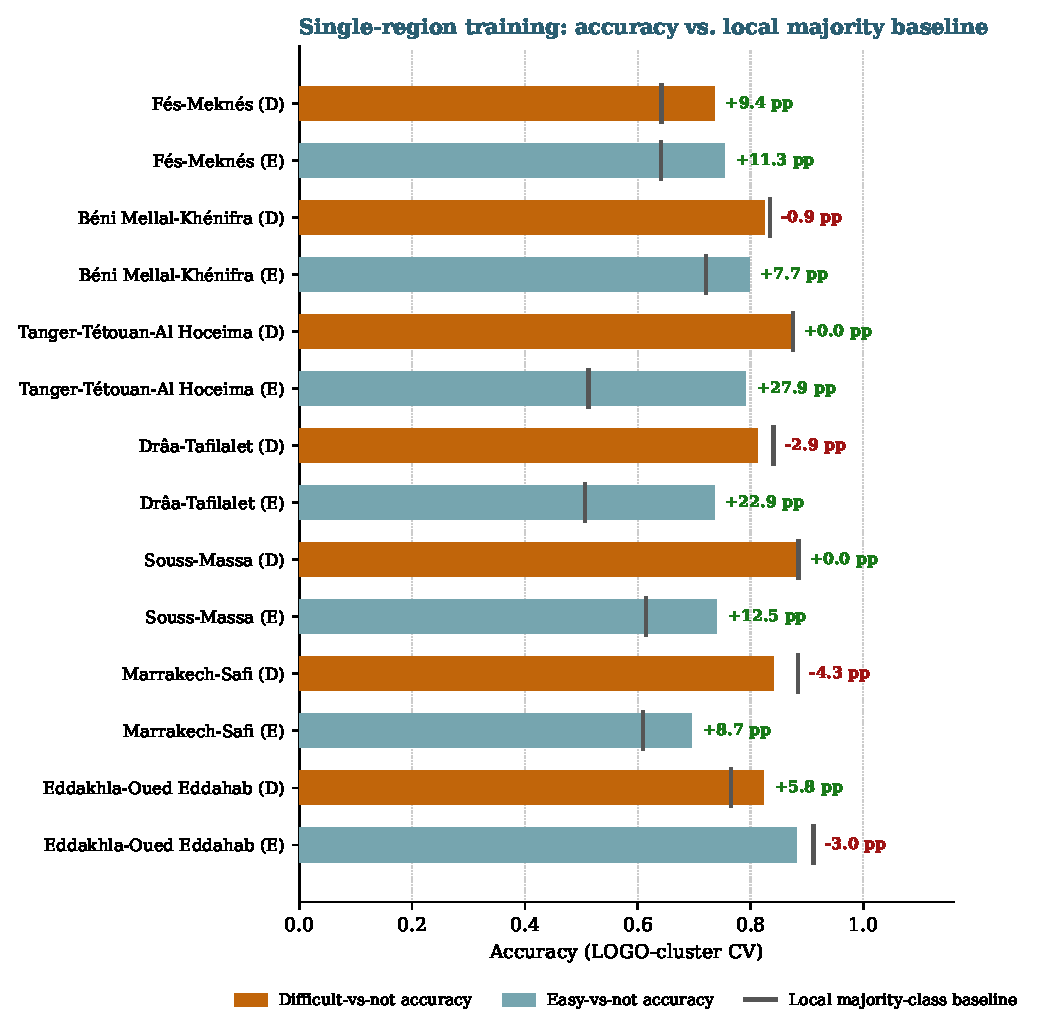
\includegraphics[width=0.92\linewidth]{figures/paper2_gap_chart_single.pdf}
\caption{Single-region training: accuracy vs.\ local majority baseline, seven individually-modeled regions, both targets.}
\label{fig:gap-single}
\end{figure}

Nine of the fourteen region/target combinations in Table~\ref{tab:region-overview} beat their local majority baseline; five do not (Béni Mellal-Khénifra Difficult, Tanger-Tétouan-Al Hoceima Difficult, Drâa-Tafilalet Difficult, Marrakech-Safi Difficult, and Eddakhla-Oued Eddahab Easy -- see Figure~\ref{fig:gap-single} for the exact gaps) -- every one of these is a case where the region's own majority class is already very high (0.76--0.91), leaving little headroom for any model to add value, and four of the five are the Difficult target specifically, consistent with the mechanism traced in Section~\ref{sec:robustness}.

\textbf{Why three regions are missing from Table~\ref{tab:region-overview} and Figure~\ref{fig:gap-single}.} Guelmim-Oued Noun ($N=7$), Laâyoune-Sakia El Hamra ($N=15$), and Casablanca-Settat ($N=7$) each carry too few labeled sites to fit a region-specific model at all -- with only 7 total sites, for instance, even a single leave-one-cluster-out fold can remove most of the positive class entirely, making any accuracy number from such a fit meaningless. Section~\ref{sec:merging} merges each of these three with a geographic neighbor instead of omitting them; their results appear only in the next subsection, as part of a merged group.

\subsection{Merged/Multi-Region Results}
\label{sec:merging}
Three regions carry too few labeled sites to model individually (previous subsection). Rather than omit them, each is merged with a geographic neighbor into a combined group large enough to fit: Guelmim-Oued Noun with Laâyoune-Sakia El Hamra (and, as a further check, that pair with Eddakhla-Oued Eddahab added), and Rabat-Salé-Kénitra with Casablanca-Settat. This is disclosed as a deliberate trade-off -- a merged group is not the same object as a single administrative region -- made specifically to get a usable result rather than three unusable ones. Table~\ref{tab:region-overview-merged} and Figure~\ref{fig:gap-merged} report these merged results the same way as the single-region ones above. Section~\ref{sec:mosaic} additionally resolves, for the final national map, which configuration (a single merged model, versus each sub-region modeled on its own) best represents each such zone.

\begin{table}[H]
\centering\footnotesize
\caption{Merged/multi-region training: best result per merged group, both binary targets. Columns as in Table~\ref{tab:region-overview}.}
\label{tab:region-overview-merged}
\begin{tabular}{@{}lrrlr@{}}
\toprule
Region group & $N$ & Pos. & Best feature set & Acc. \\
\midrule
Guelmim + Laâyoune (D) & 22 & 4 & Baseline & 0.909 \\
Guelmim + Laâyoune (E) & 22 & 9 & Baseline & 0.909 \\
Guelmim + Laâyoune + Eddakhla (D) & 55 & 12 & Baseline & 0.909 \\
Guelmim + Laâyoune + Eddakhla (E) & 55 & 12 & Baseline & 0.855 \\
Rabat-Salé-Kénitra + Casablanca-Settat (D) & 28 & 4 & +Domain & 0.821 \\
Rabat-Salé-Kénitra + Casablanca-Settat (E) & 28 & 10 & +Infra & 0.786 \\
\bottomrule
\end{tabular}

\vspace{2pt}
\noindent{\footnotesize D = Difficult-vs-not, E = Easy-vs-not. Source: \texttt{results/json/training/phase5\_paper2\_merged\_regions\_results.json}.}
\end{table}

\begin{figure}[H]
\centering
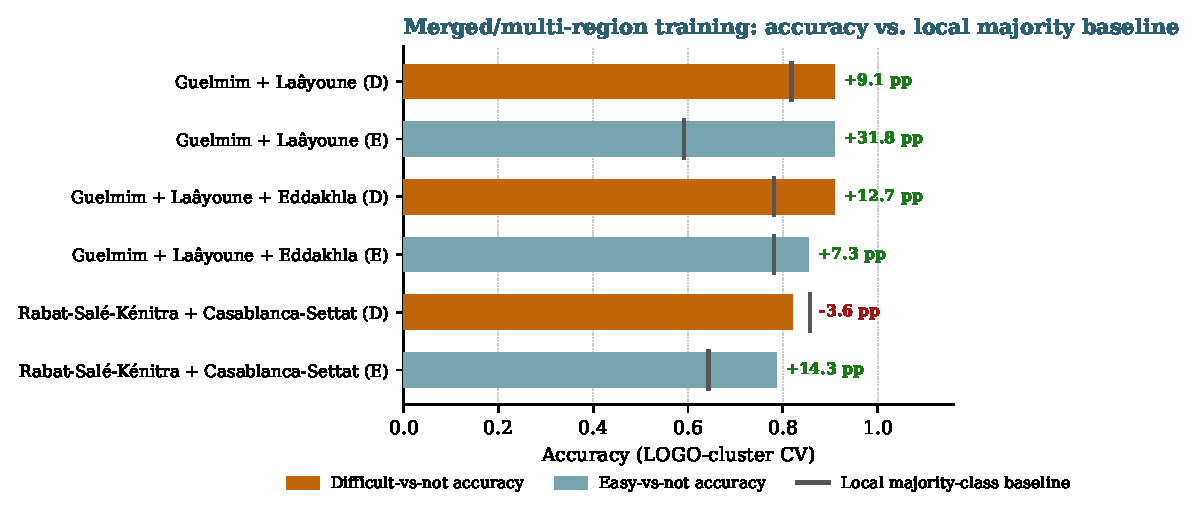
\includegraphics[width=0.92\linewidth]{figures/paper2_gap_chart_merged.pdf}
\caption{Merged/multi-region training: accuracy vs.\ local majority baseline, the three merged groups, both targets.}
\label{fig:gap-merged}
\end{figure}

Five of the six merged-group combinations beat their local majority baseline, several by a wide margin (Guelmim+Laâyoune Easy +31.8\,pp); only Rabat-Salé-Kénitra+Casablanca-Settat Difficult does not ($-$3.6\,pp), again the Difficult target specifically. Combined with the previous subsection, fourteen of the twenty region/target combinations tested in this paper beat their local majority baseline overall.

\subsection{Region-by-Region Detail}
\label{sec:region-detail}
Each region below is discussed on its own terms: what its labeled data looks like, which feature set won and why that is plausible given the region's terrain and infrastructure character, what the result does and does not establish, and its own projected map. Where a region's winning feature set is +Domain, or where +Infra grid extraction failed under the memory cap used for the country-scale OSM processing in this project (Section~\ref{sec:mosaic-limits}), the \emph{map} is rendered from the Baseline feature set instead -- disclosed explicitly per region below -- while the accuracy numbers reported in Tables~\ref{tab:region-overview}--\ref{tab:region-overview-merged} and Figures~\ref{fig:gap-single}--\ref{fig:gap-merged} always reflect the true winning variant. Geological domain has no continuous spatial raster in this project (it is a curated per-locality label, not derived from any geology shapefile), so +Domain-winning targets are always map-substituted; +Infra substitution occurs only where the region-scale POI/settlement extraction hit the processing memory cap.

\textbf{Fés-Meknés ($N=337$, largest region).} Spans the Fés-Boulemane plateau, Middle Atlas foothills, and lowland plains -- the most heterogeneous single region in the dataset, and historically the source of 72\% of the original batch's Difficult labels (Section~\ref{sec:robustness}), meaning this region's own terrain-difficulty relationship is what the national pooled model has learned best. The tourism-infrastructure feature set delivers this paper's largest single Difficult-class gain (+16.3\,pp over baseline), plausible given the region's genuinely uneven tourism development between its plateau towns and remoter Middle Atlas approaches -- exactly the kind of variation straight-line road distance alone cannot see. Easy stays with the plain baseline (+3.8\,pp); the six terrain/road features already capture most of what distinguishes an easy site here. Both targets' maps use their true winning feature set (Infra, Baseline) with no substitution.

\begin{figure}[H]
\centering
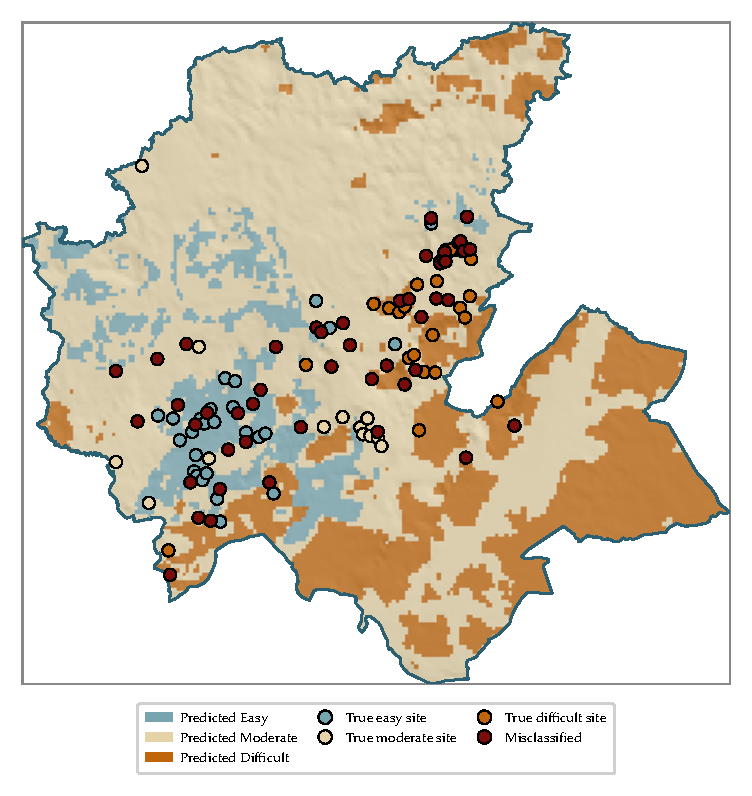
\includegraphics[width=0.5\linewidth]{figures/map_region_fesmeknes.pdf}
\caption{Fés-Meknés: projected 3-class accessibility map (Difficult: +Infra, acc.\ 0.691; Easy: Baseline, acc.\ 0.777).}
\end{figure}

\textbf{Béni Mellal-Khénifra ($N=174$).} Combines High Atlas relief with the Tadla plain, and carries the smallest Difficult-class sample of the seven individually-modeled regions ($n=19$). Even the best available feature set (geological domain) does not quite clear the local majority baseline for Difficult ($-$0.6\,pp) -- consistent with this region's karst caves and river-canyon sites, several of which sit geographically close to roads yet require technical approach that none of the three feature sets tested can represent. The Easy classifier tells a different story: tourism-infrastructure features produce a large, genuine gain (+14.9\,pp), the region's accessible Tadla-plain sites evidently correlating well with real nearby services. The Difficult map substitutes Baseline for the true winning +Domain variant (no continuous domain raster available); the Easy map uses its true winning +Infra variant directly.

\begin{figure}[H]
\centering
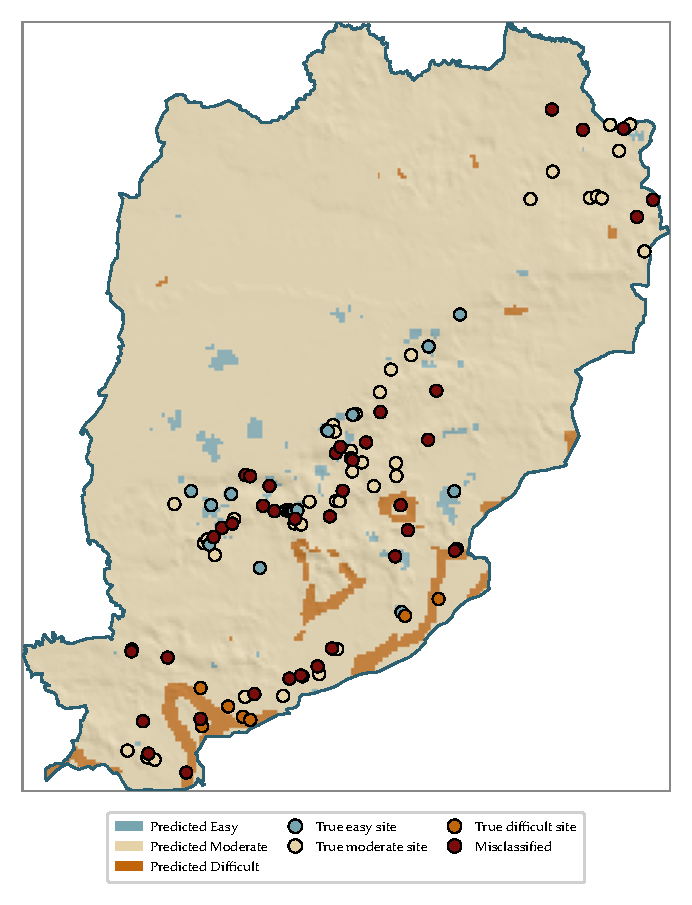
\includegraphics[width=0.5\linewidth]{figures/map_region_bmk.pdf}
\caption{Béni Mellal-Khénifra: projected map (Difficult map shown with Baseline features, substituting for the true winning +Domain variant, acc.\ 0.885; Easy: +Infra, acc.\ 0.839).}
\end{figure}

\textbf{Tanger-Tétouan-Al Hoceima ($N=128$, more than doubled since the previous labeling round: 52$\to$128 sites, 6$\to$21 Difficult).} Large enough now, for the first time, to support its own region-specific model. Geological domain is the best feature set for both targets, but the Difficult result ties the local majority baseline exactly (0.0\,pp gap) -- the region's substantial growth in labeled data did not, on its own, translate into a model that beats simply guessing the majority class, a finding worth flagging honestly rather than reporting the raw accuracy number without this context. Both targets' maps substitute Baseline for the true winning +Domain variant.

\begin{figure}[H]
\centering
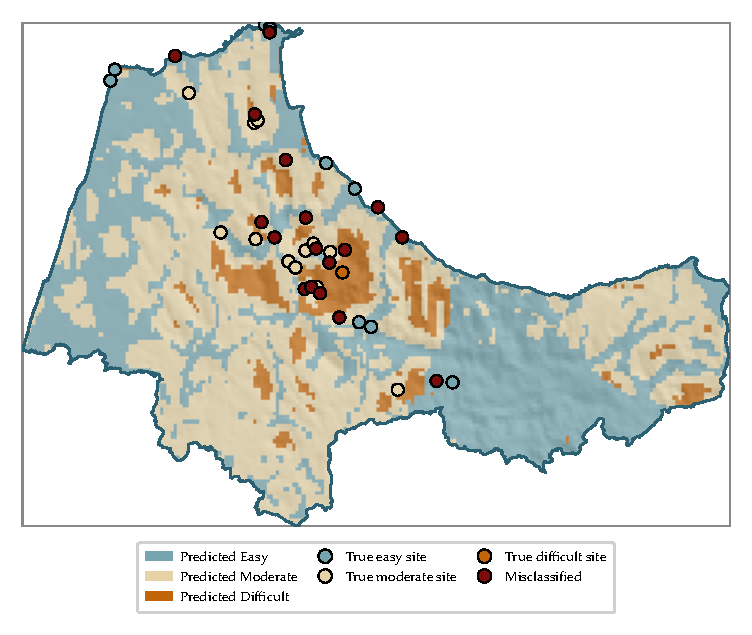
\includegraphics[width=0.5\linewidth]{figures/map_region_ttah.pdf}
\caption{Tanger-Tétouan-Al Hoceima: projected map (both targets shown with Baseline features, substituting for the true winning +Domain variant: Difficult acc.\ 0.836; Easy acc.\ 0.734).}
\end{figure}

\textbf{Drâa-Tafilalet ($N=92$, mixed environment).} The region used to test and reject the terrain-regime hypothesis (Section~\ref{sec:robustness}). Tourism-infrastructure features win both targets, with a striking asymmetry: Easy improves substantially (+15.2\,pp) while Difficult, even with the same winning feature set, still falls just short of its local majority ($-$1.1\,pp) -- the clearest single-region illustration in this paper that the same feature addition can genuinely help one target while leaving the other's underlying difficulty unresolved. This region's tourism-POI/settlement grid extraction hit the project's 4\,GB memory cap under this territory's OSM data volume; both maps are therefore shown with Baseline features, a disclosed, graceful degradation (Section~\ref{sec:mosaic-limits}) rather than a silent substitution, with the true +Infra accuracy still reported in Table~\ref{tab:region-overview}.

\begin{figure}[H]
\centering
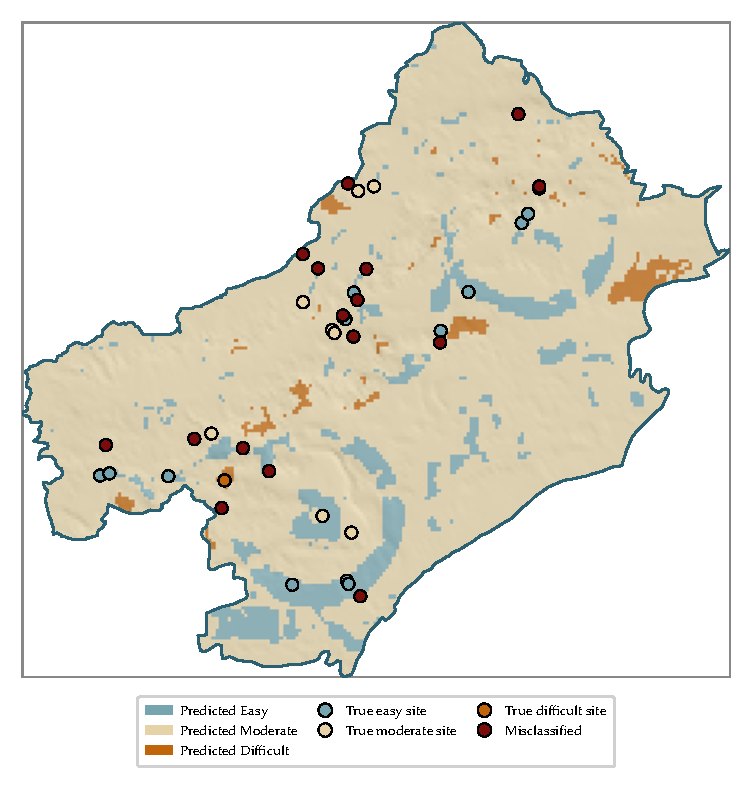
\includegraphics[width=0.5\linewidth]{figures/map_region_draa.pdf}
\caption{Drâa-Tafilalet: projected map (both targets shown with Baseline features; grid-level +Infra extraction failed under the memory cap for this territory, see text. True +Infra accuracy: Difficult 0.772; Easy 0.772).}
\end{figure}

\textbf{Souss-Massa ($N=67$).} Neither of the two engineered feature sets improves on the plain six-feature baseline for either target here; Difficult ties its local majority exactly (thin positive class, $n=7$), Easy shows a modest, real-looking gain (+4.4\,pp). A region where the baseline terrain/road features already do as well as anything else tested. Both maps use the true winning Baseline variant directly, no substitution.

\begin{figure}[H]
\centering
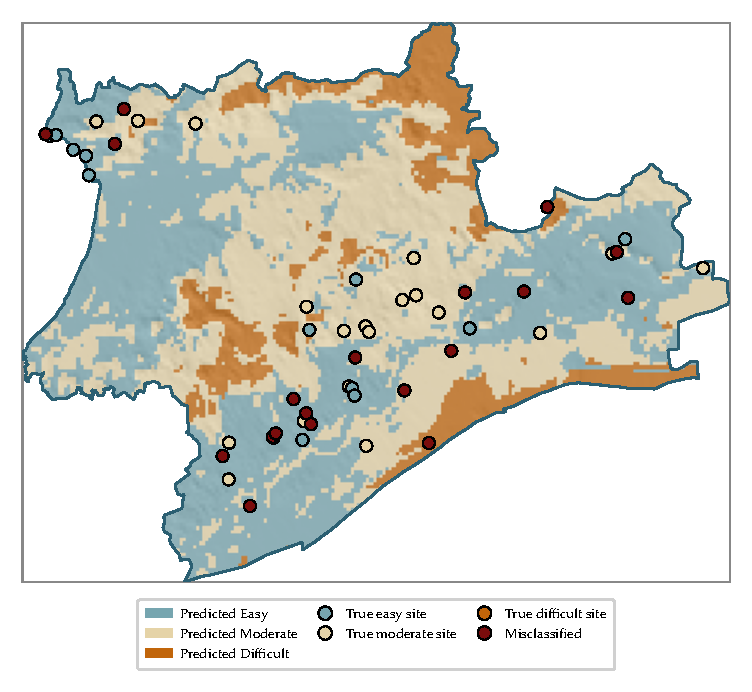
\includegraphics[width=0.5\linewidth]{figures/map_region_soussmassa.pdf}
\caption{Souss-Massa: projected map (both targets: Baseline; Difficult acc.\ 0.896; Easy acc.\ 0.701).}
\end{figure}

\textbf{Marrakech-Safi ($N=58$).} The starkest split in this paper. Easy reaches this paper's second-largest gain (+19.0\,pp, plain baseline, no feature engineering needed), while Difficult is this paper's \emph{worst} result even after trying all three feature sets ($-$10.3\,pp -- the best available option, tourism infrastructure, still falls well short of simply guessing not-Difficult). With only 8 Difficult-labeled sites in this region, this result should be read as a region where the Difficult class specifically remains essentially unmodeled with current data and features, not as a settled finding. This region's +Infra grid extraction also hit the memory cap; the Difficult map is shown with Baseline features (disclosed substitution), the Easy map with its true winning Baseline variant directly.

\begin{figure}[H]
\centering
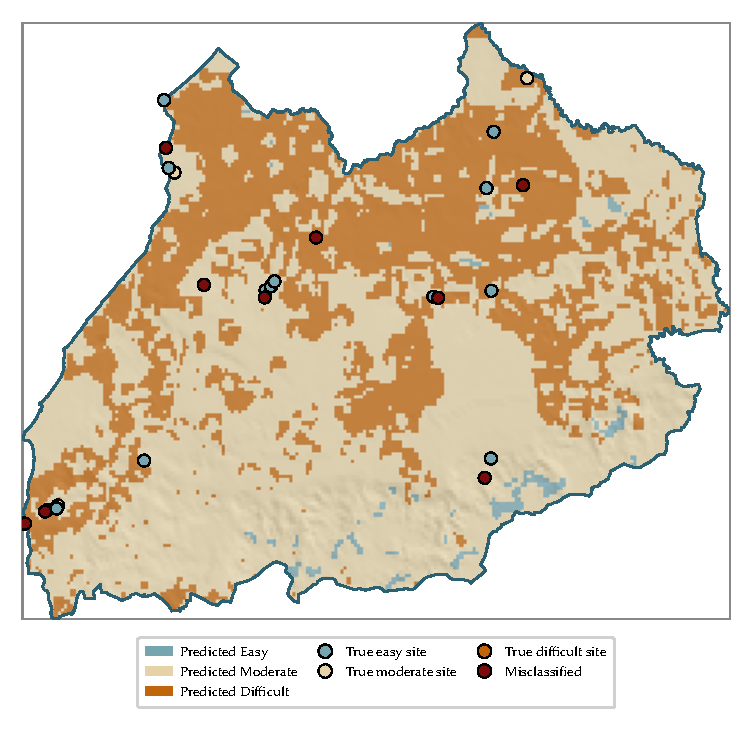
\includegraphics[width=0.5\linewidth]{figures/map_region_marrakech.pdf}
\caption{Marrakech-Safi: projected map (Difficult map shown with Baseline features, substituting for the true winning +Infra variant after grid extraction failed for this territory, acc.\ 0.759; Easy: Baseline, true winner, acc.\ 0.793).}
\end{figure}

\textbf{Eddakhla-Oued Eddahab ($N=33$).} Flat, arid, low-relief Saharan coastal terrain, previously this project's single strongest result under a national leave-region-out evaluation. Under this paper's own-region modeling, tourism infrastructure produces a real Difficult-class gain (+9.1\,pp); Easy has only 3 positive examples in the entire region, too few for any feature set to move meaningfully beyond the baseline's near-majority result ($-$3.0\,pp) -- see also Section~\ref{sec:per-algorithm}'s LightGBM finding on this exact region/target. Both maps use their true winning variant directly, no substitution.

\begin{figure}[H]
\centering
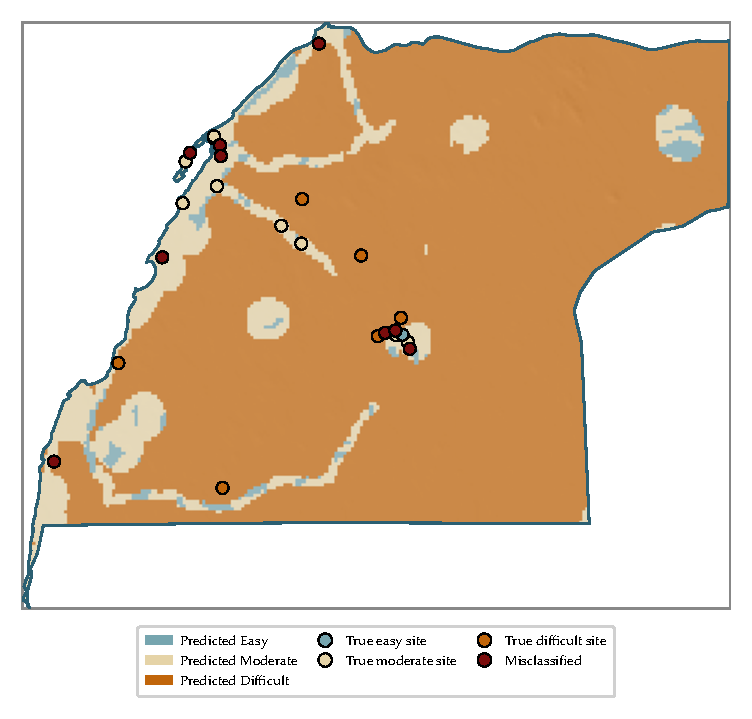
\includegraphics[width=0.5\linewidth]{figures/map_region_eddakhla.pdf}
\caption{Eddakhla-Oued Eddahab: projected map (Difficult: +Infra, acc.\ 0.849; Easy: Baseline, acc.\ 0.879).}
\end{figure}

\textbf{Guelmim-Oued Noun + Laâyoune-Sakia El Hamra ($N=22$, merged).} Individually $N=7$ and $N=15$ -- too thin to model at all. Merged, the plain baseline wins both targets outright, with Easy showing this entire paper's largest gain (+31.8\,pp): a result that did not exist in any usable form before merging, not a small improvement on an existing one. Both maps use the true winning Baseline variant directly.

\begin{figure}[H]
\centering
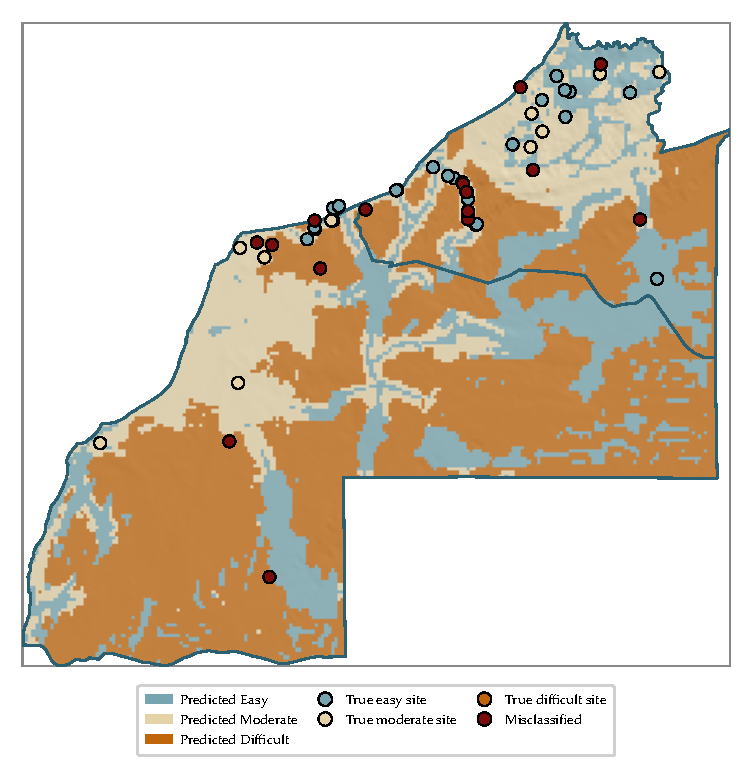
\includegraphics[width=0.5\linewidth]{figures/map_region_south_duo.pdf}
\caption{Guelmim-Oued Noun + Laâyoune-Sakia El Hamra: projected map (both targets: Baseline; Difficult acc.\ 0.909; Easy acc.\ 0.909).}
\end{figure}

\textbf{Guelmim-Oued Noun + Laâyoune-Sakia El Hamra + Eddakhla-Oued Eddahab ($N=55$, merged).} Adding Eddakhla to the pair above triples the sample size and confirms the pattern holds at larger $N$: both targets still beat their local majority substantially (+12.7\,pp, +7.3\,pp) with the plain baseline, suggesting the smaller pair's result was not a small-sample artifact. This trio configuration is evaluated here as a numeric comparison point only (Table~\ref{tab:region-overview-merged}, Figure~\ref{fig:gap-merged}); no map is shown for it. As Section~\ref{sec:mosaic} shows, its true 3-class accuracy (0.764) is an \emph{exact tie} with modeling the duo and Eddakhla independently (their own maps, previous two figures) -- the independent configuration is what the mosaic actually uses, kept for finer per-territory modeling rather than for any accuracy advantage, since there isn't one.

\textbf{Rabat-Salé-Kénitra + Casablanca-Settat ($N=28$, merged).} A more mixed result than the southern merge: geological domain lifts Difficult but still leaves it short of the local majority ($-$3.6\,pp), while tourism-infrastructure features deliver a solid Easy-class gain (+14.3\,pp) -- broadly consistent with the Difficult/Easy asymmetry seen across most other regions in this paper. The Difficult map substitutes Baseline for the true winning +Domain variant; the Easy map's +Infra grid extraction hit the memory cap, so it too is shown with Baseline.

\begin{figure}[H]
\centering
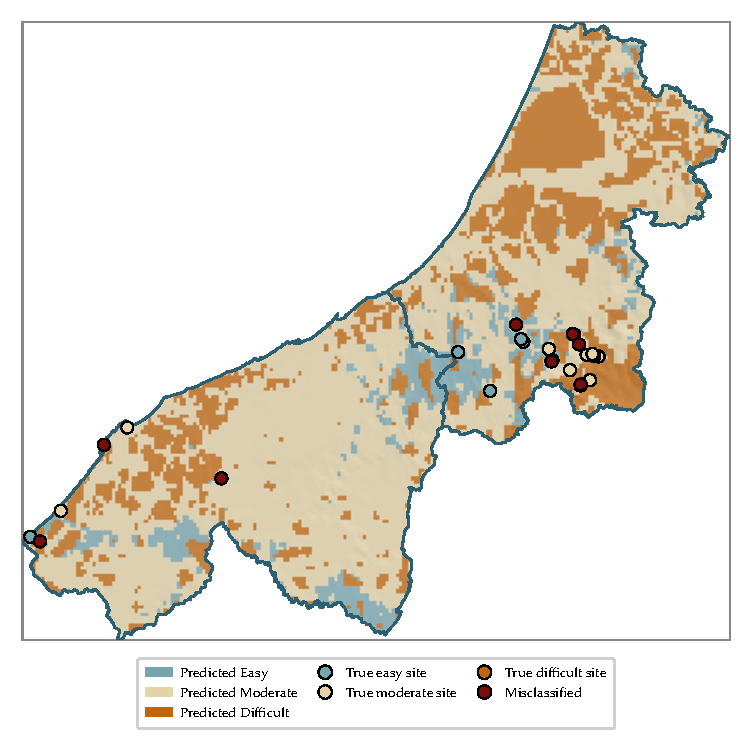
\includegraphics[width=0.5\linewidth]{figures/map_region_rabatcasa.pdf}
\caption{Rabat-Salé-Kénitra + Casablanca-Settat: projected map (Difficult map shown with Baseline features, substituting for the true winning +Domain variant, acc.\ 0.821; Easy map shown with Baseline features, substituting for the true winning +Infra variant after grid extraction failed for this territory, acc.\ 0.786).}
\end{figure}

\subsection{Per-Algorithm Comparison}
\label{sec:per-algorithm}
Table~\ref{tab:per-algorithm} breaks out each region's four tree/boosting algorithms individually, on the six-feature baseline, rather than the soft-voted ensemble reported above -- the explicit comparative view requested for this paper.

\begin{table}[H]
\centering\footnotesize
\caption{Random Forest / XGBoost / Gradient Boosting / LightGBM, individually, per region and target (six-feature baseline, 500\,m LOGO-cluster CV). Ensemble column is the four-model soft vote reported in Table~\ref{tab:region-overview}'s Baseline rows for reference.}
\label{tab:per-algorithm}
\begin{tabular}{@{}lrrrrr@{}}
\toprule
Region (target) & RF & XGB & GBM & LightGBM & Ensemble \\
\midrule
Fés-Meknés (D) & 0.671 & 0.650 & 0.647 & 0.647 & 0.671 \\
Fés-Meknés (E) & 0.777 & 0.748 & 0.769 & 0.733 & 0.777 \\
Béni Mellal-Khénifra (D) & 0.862 & 0.897 & 0.874 & 0.885 & 0.868 \\
Béni Mellal-Khénifra (E) & 0.741 & 0.736 & 0.776 & 0.787 & 0.799 \\
Tanger-Tétouan-Al Hoceima (D) & 0.820 & 0.797 & 0.844 & 0.805 & 0.812 \\
Tanger-Tétouan-Al Hoceima (E) & 0.758 & 0.672 & 0.766 & 0.742 & 0.719 \\
Drâa-Tafilalet (D) & 0.696 & 0.707 & 0.696 & 0.674 & 0.707 \\
Drâa-Tafilalet (E) & 0.674 & 0.696 & 0.707 & 0.609 & 0.761 \\
Souss-Massa (D) & 0.836 & 0.821 & 0.821 & 0.731 & 0.896 \\
Souss-Massa (E) & 0.627 & 0.672 & 0.612 & 0.642 & 0.701 \\
Marrakech-Safi (D) & 0.776 & 0.724 & 0.793 & 0.707 & 0.707 \\
Marrakech-Safi (E) & 0.724 & 0.724 & 0.741 & 0.707 & 0.793 \\
Eddakhla-Oued Eddahab (D) & 0.879 & 0.818 & 0.727 & 0.758 & 0.788 \\
Eddakhla-Oued Eddahab (E) & 0.848 & 0.879 & 0.879 & \textbf{0.000} & 0.879 \\
\bottomrule
\end{tabular}

\vspace{2pt}
\noindent{\footnotesize D = Difficult-vs-not, E = Easy-vs-not. Source: \texttt{results/json/training/phase5\_per\_algorithm\_regional\_results.json}.}
\end{table}

The bolded LightGBM$=0.000$ entry (Eddakhla-Oued Eddahab, Easy, $N=33$, only 3 positive examples) is a genuine, reproduced result, not a script defect: with class-balance weighting giving the 3 positive training examples roughly 10.7$\times$ the weight of the rest, this specific LightGBM configuration learns to predict Easy almost everywhere in every fold except the exact folds containing a true Easy site, where it flips to predicting Not-Easy -- perfectly anti-correlated with ground truth by unlucky construction, and confirmed identical across repeated runs. Random Forest, XGBoost, and Gradient Boosting on the exact same 33-site split all land in a normal 0.73--0.88 range. This is disclosed as a specific robustness limitation of one algorithm under extreme class imbalance at very small $N$, not corrected or excluded after the fact -- the four-model soft-voted ensemble reported elsewhere in this paper is unaffected here because it averages across all four, diluting one algorithm's collapse rather than being blind to it.

\subsection{National Mosaic Map}
\label{sec:mosaic}
Figure~\ref{fig:mosaic} assembles the per-region and per-merged-group maps of Section~\ref{sec:region-detail} into a single national-extent map, each zone shaded by its own best-performing model rather than one pooled national model, with regional administrative borders overlaid.

\begin{figure}[H]
\centering
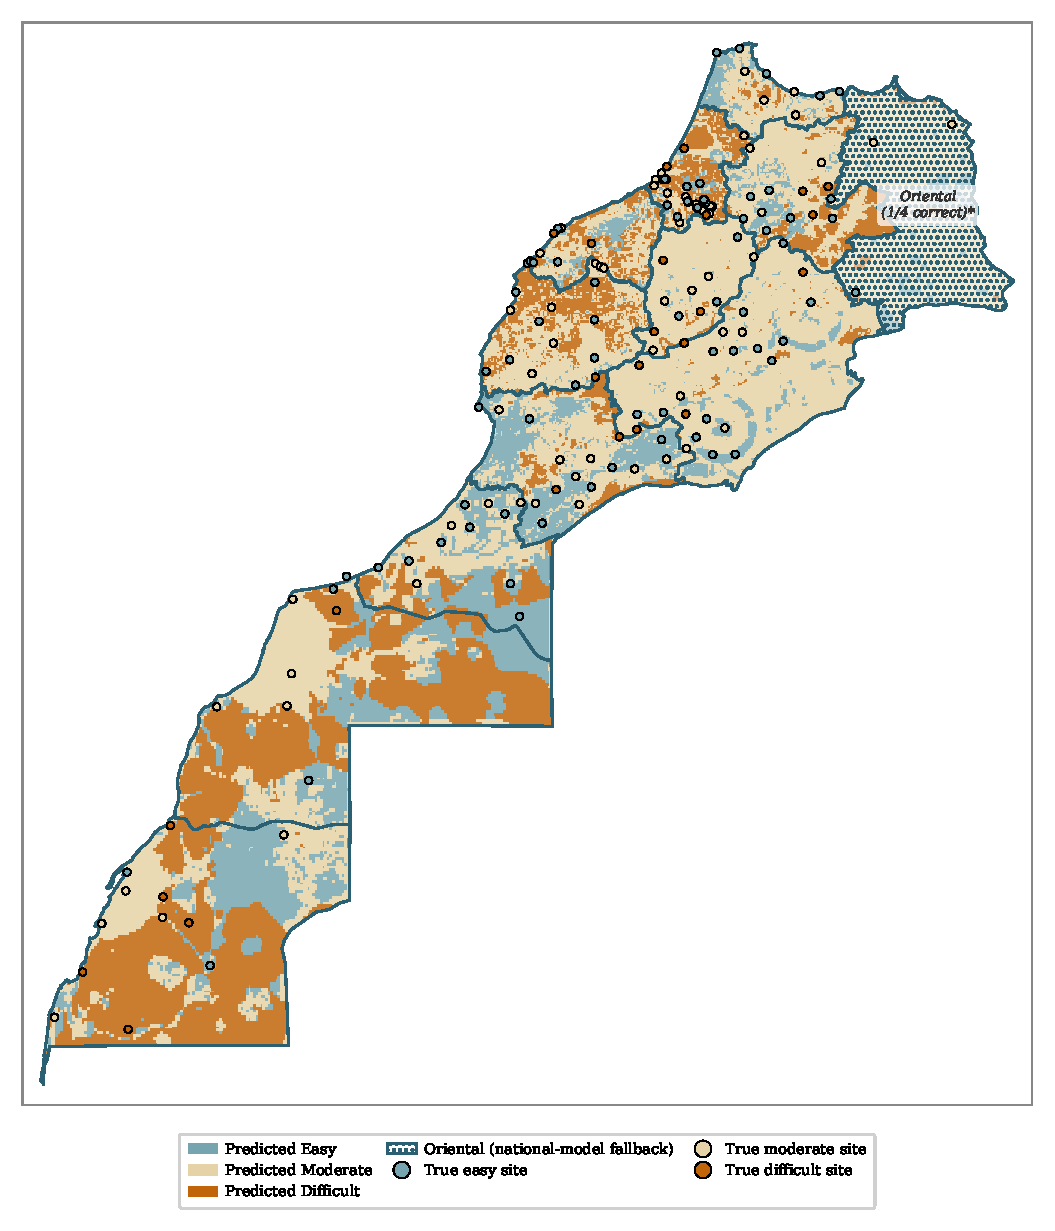
\includegraphics[width=0.62\linewidth]{figures/map_national_mosaic.pdf}
\caption{National mosaic: each of eleven regions/merged zones shaded by its own best-performing region-specific model. Oriental (grey, hatched) carries zero labeled geosites in the catalog and is not modeled -- shown as missing data, not filled from a national fallback model. Known-geosite overlay and misclassification rings as in the per-region maps.}
\label{fig:mosaic}
\end{figure}

\textbf{Zone-composition decisions.} Two of the eleven modeled zones had more than one candidate configuration available (Section~\ref{sec:methodology}), and the choice for each was resolved quantitatively rather than by default:

\emph{South zone (Guelmim-Oued Noun, Laâyoune-Sakia El Hamra, Eddakhla-Oued Eddahab).} Using each configuration's true per-site LOGO-cluster CV out-of-fold prediction (the same ground truth used for the ring markers throughout this paper), the trio configuration's own 3-class accuracy across its 55 sites is $42/55 = 0.764$. The alternative -- Guelmim+Laâyoune modeled independently from Eddakhla -- gives a sample-weighted accuracy of $(18+24)/55 = 0.764$ (duo: 18/22 correct; Eddakhla-standalone: 24/33 correct) -- an exact tie with the trio, not an improvement on it. The independent configuration was kept for the mosaic regardless, since it gives finer per-territory modeling at no accuracy cost, not because it outperforms the trio; the trio's own map is still shown in Section~\ref{sec:region-detail} for comparison, since it remains an equally valid result, just not the one used here.

\emph{Rabat-Salé-Kénitra + Casablanca-Settat.} No standalone alternative exists for this zone as a whole: Casablanca-Settat was never fit standalone ($N=7$, too thin -- the reason this merge exists at all), and Rabat-Salé-Kénitra's own Difficult target is degenerate standalone (only 2 Difficult-labeled sites once the 21-site region is isolated). A direct comparison was still run for the one target where an alternative existed, Easy, refitting both Rabat-standalone's and the merged pair's winning configurations with per-site out-of-fold predictions and evaluating both restricted to Rabat's own 21 sites (the fair, apples-to-apples test, since the merged model is trained on more data but only this subset is common ground): Rabat-standalone reaches 0.8095, the merged model restricted to the same 21 sites also reaches 0.8095 -- an exact tie. Given the tie, and that the merged model is the only configuration with full coverage of both territories, the merged configuration was used for the mosaic across the whole zone (Source: \texttt{data\_audit/28\_paper2\_rabatcasa\_zone\_compare.py}, \texttt{results/json/other/phase5\_paper2\_rabatcasa\_zone\_comparison.json}).

\textbf{Coverage and limitations.}
\label{sec:mosaic-limits}
The mosaic covers eleven of Morocco's twelve regions and all 939 labeled sites in the catalog. Oriental is shown as missing data rather than modeled from any national or neighboring-region fallback, per an explicit decision to disclose the gap honestly rather than paper over it with an unvalidated extrapolation: the underlying labeled catalog contains zero geosites for this region, so there is no ground truth against which any model covering it could even be checked. Within the eleven modeled zones, four region/target combinations (Béni Mellal-Khénifra Difficult, Tanger-Tétouan-Al Hoceima both targets, Drâa-Tafilalet both targets, Marrakech-Safi Difficult, Rabat-Salé-Kénitra+Casablanca-Settat both targets) have their \emph{map} rendered with Baseline features substituting for a true winning +Domain or +Infra variant (Section~\ref{sec:region-detail} discloses each individually); the underlying accuracy numbers in Tables~\ref{tab:region-overview}--\ref{tab:region-overview-merged} always reflect the true winning variant regardless of what the map shows. Overall, across the 939 sites shown on the mosaic, 339 (36.1\%) are misclassified by the combined 3-class decision rule (per-site LOGO-cluster CV out-of-fold predictions, exactly matching the accuracy numbers in Tables~\ref{tab:region-overview}--\ref{tab:region-overview-merged}) -- consistent with, not worse than, the per-region 3-class misclassification rates already visible in Section~\ref{sec:region-detail}'s individual maps, since the mosaic is a direct assembly of those same per-region rasters rather than a new, separately-fit model.

\section{Robustness and Limitations}
\label{sec:robustness}
This section reports five findings from a deliberate, systematic robustness investigation -- not incidental observations, but the direct product of testing and, where warranted, ruling out five separate candidate explanations for why the Difficult class specifically underperforms across most regions.

\textbf{The dominant, evidenced cause: one region's terrain signature standing in for the whole labeled Difficult class.} Of the original 733-site labeled batch, 72\% of all Difficult-labeled sites (155 of 215) come from Fés-Meknés alone. A model trained on this pool learns, in large part, the Fés-Meknés-specific relationship between terrain/road proximity and difficulty (a mountain-terrain, moderate-road-distance signature) rather than a general one. Directly testing this: on the original batch, Difficult precision is 0.650 in Fés-Meknés but only 0.417 in every \emph{other} region combined ($N=411$, 14.6\% Difficult prevalence there versus 47.2\% in Fés-Meknés) -- and this same low-precision pattern (0.265) recurs in the entirely separate, independently-labeled 206-site batch (17.0\% Difficult prevalence), which is not concentrated in Fés-Meknés at all. Two batches from different labelers, sharing only the same low local Difficult prevalence, show the same failure -- ruling out labeler-specific error as the cause and confirming a base-rate/threshold-calibration mechanism: a single global decision threshold, implicitly tuned to Fés-Meknés' unusually high 47\% Difficult rate, over-predicts Difficult wherever the true local rate is much lower, producing exactly the false-positive-heavy precision collapse observed.

\textbf{A terrain-regime explanation was tested and specifically ruled out.} Before settling on the prevalence mechanism above, an elevation/road-distance ``regime split'' hypothesis (mountain-near-road versus remote-lowland difficulty as two distinct terrain mechanisms) was tested directly by splitting all Difficult sites into two regimes using the newer batch's own observed median elevation and highway-distance values. Properly measured with precision and recall rather than raw accuracy, the remote-lowland regime performed \emph{as well or slightly better} than the mountain regime (precision 0.603 vs.\ 0.500), the opposite of what the terrain-regime hypothesis predicted -- this candidate explanation is reported here specifically because it was refuted by evidence, not because it confirmed anything, consistent with reporting negative results rather than only positive ones.

\textbf{Cross-region generalization is weak almost everywhere, independent of feature set.} Leave-region-out testing (training on all other regions, zero exposure to the target region) was run for the two regions carrying the strongest theoretical interest: Tanger-Tétouan-Al Hoceima and Souss-Massa, using a road-network routing-distance feature (true shortest-path distance along the OSM road graph, not straight-line) in place of the standard straight-line highway-distance feature. Pooled across these two regions, the routing feature produces a statistically confirmed accuracy gain over the straight-line baseline (+8.7 percentage points, McNemar $\chi^2=8.26$, $p=0.004$) -- but when the identical test is repeated across every region with a usable leave-region-out sample, the pooled effect is not significant ($p=0.276$): the routing feature helps Tanger-Tétouan-Al Hoceima (+7.0\,pp) and Souss-Massa (+11.9\,pp) specifically, is flat in most other regions, and actively hurts Eddakhla-Oued Eddahab ($-$9.1\,pp). The honest reading is that road-network routing distance is a real, regionally-selective improvement, not a general cross-region generalization fix, and should not be reported as either.

\textbf{Algorithm choice is a smaller factor than feature-set and regional context.} Section~\ref{sec:per-algorithm}'s per-algorithm table shows individual tree/boosting algorithms varying by up to 15--20 percentage points within the same region and target (e.g.\ Marrakech-Safi Difficult: XGBoost 0.724 vs.\ Gradient Boosting 0.793), but this variance is smaller and less systematic than the variance driven by feature-set choice (Table~\ref{tab:region-overview}) or by which region is being modeled at all -- consistent with the national companion paper's model-family comparison (logistic regression, $k$-NN, Gaussian Process), where none of four additional model families displaced the deployed tree ensemble by a confirmed margin either.

\textbf{Hyperparameter selection is not fully nested within the outer cross-validation.} As in the national companion paper: for each reported model, the best configuration among Random Forest/XGBoost/Gradient Boosting/LightGBM (and, here, the best of three feature-set variants) is chosen once via grid search on the full regional dataset, then reused across every fold of the outer leave-one-group-out evaluation that produces the headline accuracy. This is a common simplification in applied work, not full nested cross-validation, disclosed here rather than treated as fully addressed -- and is a larger concern at the region-specific scale of this paper than nationally, since smaller $N$ per region gives model selection relatively more of the total sample to have already seen.

\section{Conclusion}
Applying the same feature stack and validation protocol used nationally, region by region, with each region allowed its own best-performing feature set among three candidates, shows a genuinely uneven picture: fourteen of twenty region/target combinations beat their local majority-class baseline, several by a wide margin (Marrakech-Safi Easy +19.0\,pp, the merged Guelmim-Oued Noun/Laâyoune-Sakia El Hamra group +31.8\,pp on the same target), while six do not clear their local baseline even with the best available feature set -- concentrated, not coincidentally, in the Difficult class. That concentration is traced to a specific, evidenced mechanism rather than left as an unexplained weakness: one region's terrain signature (Fés-Meknés, 72\% of the original Difficult-labeled training pool) implicitly sets the model's decision threshold, which then over-predicts Difficult wherever the true local rate is much lower -- confirmed independently across two separately-labeled batches, and distinguished from two ruled-out alternative explanations (a terrain-regime split, and a batch-quality difference) tested and rejected along the way. Three regions individually too thin to model become usable once merged with a geographic neighbor, and a road-network routing-distance feature is shown to help two specific regions substantially without generalizing as a fix everywhere. Every region's and merged group's result is projected onto a real geographic grid and shown as its own map, and these are combined -- with each contested zone's configuration (independent vs.\ merged) resolved by a direct, quantitative, apples-to-apples comparison rather than by default -- into a single national mosaic covering eleven of Morocco's twelve regions, the clearest visual summary this project has produced of where region-specific accessibility modeling currently works, where it does not, and why. Together with the per-algorithm comparison (Section~\ref{sec:per-algorithm}), this paper provides the detailed, region-by-region performance/robustness/limitations picture that the national companion paper's pooled figures are not designed to show, and sets up the natural next step: a focused, single-region deep dive selected from the strongest and most instructive results reported here.

\end{document}
